\documentclass{beamer}
\usepackage[latin1]{inputenc}
\usepackage{tikz}
\usepackage{makecell}
\usepackage{pgfplots}
\usepackage{pgfplotstable} 
%\pgfplotsset{compat=1.12}
\usepackage{sansmath}
\usetheme{Berlin}
\usetikzlibrary{
	arrows.meta,
	chains,
	decorations.pathreplacing,
	automata,
	positioning,
	scopes,
	quotes,
	shapes,
	shadows	
}
\title{Fast Decompression Lucene Codec}
\author{Ivan Mamontov\\ Grid Dynamics}
\institute{Berlin Buzzwords}
\date{Jun 1st, 2015}
\titlegraphic{
%	
\includegraphics[width=3.8cm]{resources/buzzwordslogo.png}			\hspace*{8.75cm}~
}


\pgfplotstableread[col sep=comma]{
a,b,c,d,e
128,  82.638  ,200.452 ,194.441  ,330.123  
256,  139.914 ,261.881 ,346.855  ,583.440  
512,  225.505 ,341.506 ,592.312  ,1046.636 
1024, 396.605 ,518.709 ,1100.371 ,2149.478 
2048, 743.370 ,868.560 ,2089.506 ,4058.115 
4096, 1436.633,1557.861,4204.929 ,8023.846 
8192, 2827.855,2953.913,7758.365 ,14458.539
16384,5654.820,5779.984,14938.887,25235.819
}\mytable

\begin{document}
	\begin{frame}
		\titlepage
	\end{frame}
	\begin{frame}
    		\begin{itemize}
    			\frametitle{About me}
    		    \item Software engineer at Grid Dynamics
    		    \item I am interested in low-level system programming
		\end{itemize}
  	\end{frame}
  	\begin{frame}
  		\frametitle{Agenda}
  			\begin{itemize}
  			\item Lucene Codecs
  			\item What is SIMD?
  			\item Java Critical
  			\item Benchmarking
  			\end{itemize}
  	\end{frame}
  	\begin{frame}
  		\frametitle{Lucene Codec}
  		\begin{itemize}
  			\item Lucene 3
  			\begin{itemize}
  				\item Tuned to pre-defined data types
  				\item Combinations of delta and variable-byte encodings
  				\item Impossible to customize
  				\item Dependencies on specific file-system behaviors
  			\end{itemize}
	  			\item Lucene 4
  					\begin{itemize}
  						\item All data writing and reading abstracted from data encoding
  						\item Highly customizable
  					\end{itemize}		
  		\end{itemize}
  	\end{frame}
  	\begin{frame}
  		\frametitle{Lucene 5.0 codec}
  		The default Lucene50 codec is:
  		\begin{itemize}
  			\item variable-byte and fixed-width encoding of delta values
  			\item multi-level skip lists
  			\item natural ordering of docIDs
  			\item encodes both term frequencies and positional information
  		\end{itemize}
  	\end{frame}

  	\begin{frame}
  		\frametitle{What is variable-byte encoding?}
  		Encode sequence of numbers into variable-length bytes using one status bit per byte indicating whether the current number expands into next byte.
  	\end{frame}
  	\begin{frame}
  		\frametitle{What is variable-byte encoding?}
  		To encode the decimal number 6917(00011011 00000101):
		\vskip15pt 
  		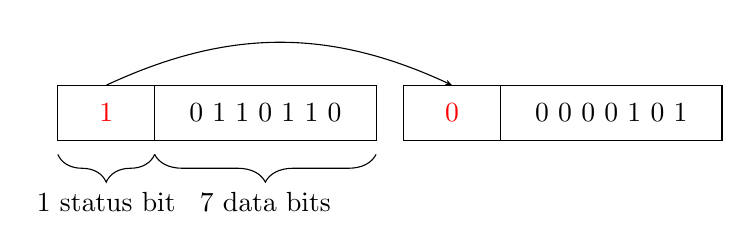
\begin{tikzpicture}[
 		      	start chain = going right,
     			node distance = 0pt,
				ArrayStyle/.style={draw, minimum width=3.5em, minimum 									height=2em, outer sep=0pt, on chain}]
			\node [ArrayStyle] (1) {{\color{red!100}1}};
			\node [ArrayStyle, minimum width=8em] (2) {0 1 1 0 1 1 0};
			\node [ArrayStyle, xshift=1em] (3) {{\color{red!100}0}};
			\node [ArrayStyle, minimum width=8em] (4) {0 0 0 0 1 0 1};
			\begin{scope}[-{Stealth[length = 2.5pt]}]
  				\draw (1.north) [out=25, in=155] to (3.north);
			\end{scope}
			\draw[decorate,decoration={brace, amplitude=10pt, 					raise=5pt, mirror}]
  				(2.south west) to node[black,midway,below= 15pt] 				{$7$ data bits} (2.south east);
			\draw[decorate,decoration={brace, amplitude=10pt, 					raise=5pt, mirror}]
  				(1.south west) to node[black,midway,below= 15pt] 				{$1$ status bit} (1.south east);
		\end{tikzpicture} 
		\vskip15pt 	
		\pause
		Thus needs 2 bytes instead of 4 bytes!
  	\end{frame}
  	\begin{frame}
  		\frametitle{What is variable-byte encoding?}
  		\begin{itemize}
    		    \item pros
    		    \begin{itemize}
    		    		\item wonderfully simple
    		    		\item good compression rate
    		    \end{itemize}
    		    \item cons
    		    \begin{itemize}
    		    		\item it requires an if statement on every byte	during decode% which is very costly since the CPU cannot easily predict the branch outcome.
    		    \end{itemize}
		\end{itemize}
  	\end{frame}
  	\begin{frame}
  		\frametitle{What is FOR encoding?}
  		Frame-of-reference encoding takes each fixed block of integers and stores them all as packed delta values, where each value gets N bits, set by the maximum delta in the block.	
  	\end{frame}
  	\begin{frame}
  		\frametitle{What is FOR encoding?}
  		To encode the following numbers 1, 3, 7, 10, 13, 14, 18:
		\vskip15pt 
  		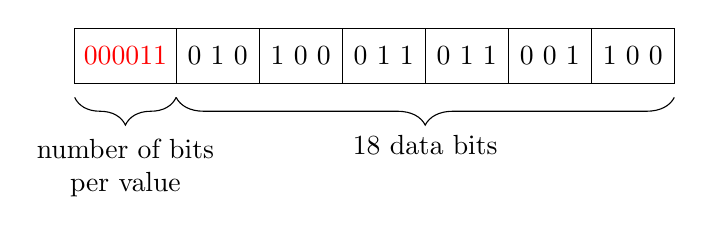
\begin{tikzpicture}[
 		      	start chain = going right,
     			node distance = 0pt,
				ArrayStyle/.style={draw, minimum width=3.5em, minimum 									height=2em, outer sep=0pt, on chain}]		
			\node [ArrayStyle] (1) {{\color{red!100}000011}};
			\node [ArrayStyle, minimum width=3em] (2) {0 1 0};
			\node [ArrayStyle, minimum width=3em] (3) {1 0 0};
			\node [ArrayStyle, minimum width=3em] (4) {0 1 1};
			\node [ArrayStyle, minimum width=3em] (5) {0 1 1};	
			\node [ArrayStyle, minimum width=3em] (6) {0 0 1};
			\node [ArrayStyle, minimum width=3em] (7) {1 0 0};	
			\draw[decorate,decoration={brace, amplitude=10pt, 					raise=5pt, mirror}]
  				(2.south west) to node[black,midway,below= 15pt] 				{18 data bits} (7.south east);
			\draw[decorate,decoration={brace, amplitude=10pt, 					raise=5pt, mirror}]
  				(1.south west) to node[black,midway,below= 15pt] 				{\makecell[c]{number of bits\\per value}} (1.south east);
		\end{tikzpicture} 
		\vskip15pt 	
		\pause
		Thus needs 3 bytes instead of $7*4=32$ bytes!
  	\end{frame}
  	\begin{frame}
  		\frametitle{What is FOR encoding?}
  		\begin{itemize}
    		    \item pros
    		    \begin{itemize}
    		    		\item two times faster during decoding than VInt % Up to 2 times faster than in variable-byte encoding
    		    		\item \textbf{can be processed using a vectorized version} (SIMD)
    		    \end{itemize}
    		    \item cons
    		    \begin{itemize}
    		    		\item in order to access even one int within the block, we must decode the full block
    		    		\item requires integers in batches of multiples of 32
    		    		\item the cost is determined by the largest delta in a block
    		    \end{itemize}
		\end{itemize}  		
  	\end{frame}
  	\begin{frame}
%With conventional scalar operations, four add instructions must be executed one after another to obtain the sums as shown
    		\frametitle{What is SIMD?}
    		Single Instruction Single Data (SISD)
    		\vskip15pt 
  		\tikzset{% define the style of the nodes for drawing the squares
     		mysquare/.style={shape=rectangle,draw=black!                       			100,thick,top color=white}
   		}

  		\begin{tikzpicture}
    			\foreach \x in {0,...,3} {% loop over the three rows
       		\node[mysquare] at (0,-\x) {$A_\x$};
       		\node at (1,-\x) {$+$};
       		\node[mysquare] at (2,-\x) {$B_\x$};
       		\node at (3,-\x) {$=$};
       		\node[mysquare] at (4,-\x) {$C_\x$};
    			}
		 \end{tikzpicture}
		
  	\end{frame}
  	\begin{frame}
    		\frametitle{What is SIMD?}
    		    Single Instruction Multiple Data (SIMD)
    		    \vskip15pt 
  			\tikzset{
     			mysquare/.style={shape=rectangle,draw=black!			                100,thick,top color=white}
   			}
		    \begin{tikzpicture}% use positioning to put the boxes together
    				\foreach \letter/\col/\x in {A/yellow!30/0, B/green!40/2, C/red!50/4} {
      				\node[mysquare=\col] (\letter 0) at (\x,0){$\letter_0$};
      				\node[below=-1pt of \letter 0,mysquare=\col] (\letter 1) {$\letter_1$};
      				\node[below=-1pt of \letter 1,mysquare=\col] (\letter 2) {$\letter_2$};
      				\node[below=-1pt of \letter 2,mysquare=\col] (\letter 3) {$\letter_3$};
    				}
    				\node at (1,-0.8) {$+$};% place + and = by hand
    				\node at (3,-0.8) {$=$};
  			\end{tikzpicture}
  	\end{frame}
  	\begin{frame}
    		\frametitle{What is SIMD?}
    		\begin{itemize}
    		    \item pros
    		    \begin{itemize}
    		    		\item 75\% fewer loads
    		    		\item 75\% fewer adds
    		    		\item 75\% fewer stores
    		    \end{itemize}
    		    \item cons
    		    \begin{itemize}
    		    		\item not all algorithms can be vectorized
    		    		\item in complicated cases compilers don't able to vectorize
    		    \end{itemize}
		\end{itemize}
  	\end{frame}  	
  	\begin{frame}[fragile=singleslide]
  		%Let us explain this with an example:
  		%The code in example 1b can be reduced to just 4 machine instructions if the
		%instruction set AVX or higher is enabled. The SSE2 instruction set will give 8
		%machine instructions because the maximum vector register size is half as big for
		%instruction sets prior to AVX. The code in example 1a will generate approximately
		%44 instructions if the compiler does not automatically vectorize the code.
    		\frametitle{What is SIMD?}
		\begin{verbatim}
float a[8], b[8], c[8];       
...
for (int i = 0; i < 8; i++) { 
 c[i] = a[i] + b[i]*1.5f;     
}
		\end{verbatim}
		\begin{itemize}
			\item JIT $\approx86$ machine instructions
			\item gcc $\approx44$ machine instructions without vectorization
			\item gcc -- 8 machine instructions with SSE2
			\item gcc -- 4 machine instructions with AVX
		\end{itemize}
  	\end{frame}  	
  	\begin{frame}
  		\frametitle{Auto-vectorization in HotSpot}
  		%Sometimes it is possible to move the kernel to C/C++, use SIMD there and call via JNI. However, the cost of the JNI call can be significant as are the difficulties of ensuring memory is properly aligned for SIMD execution
  		%In HotSpot versions beginning with Java 7u40, the server compiler provides support for auto-vectorisation. According to JDK-6340864
		%However, this seems to be true only for "simple loops" - at least for the moment. For example, accumulating an array cannot be vectorised yet JDK-7192383
		Vector arithmetic is not supported yet. Only array initialization and array copy.
  		\begin{itemize}
  			\item \url{http://bugs.java.com/view_bug.do?bug_id=6340864}
  			\item \url{http://bugs.java.com/view_bug.do?bug_id=7192383}
  		\end{itemize}
  	\end{frame}
  	\begin{frame}
  		\frametitle{Cost of JNI Call	in HotSpot}
  		\begin{itemize}
  			\item Move arguments according to ABI.
  			\item Wrap object references to JNI handles.
  			\item Obtain JNIEnv*, jclass/jobject and pass them as parameters.
  			\item Check if should call method\_entry trace function.
  			\item Lock an object monitor if the method is synchronized.
  			\item Check if the native function is linked already.%Function lookup and linking is performed lazily.
  			\item Switch thread from in\_java to in\_native state.
  			\item \textbf{Call the native function.}
  			\item Check if safepoint is needed.
  			\item Return thread to in\_java state.
  			\item Unlock monitor if locked.
  			\item Notify method\_exit.
  			\item Unwrap object result and reset JNI handles block.
  			\item Handle JNI exceptions.
  		\end{itemize}
  	\end{frame}
  	\begin{frame}
  		\frametitle{JDK-7013347 Critical Native}
  		\begin{itemize}
  			\item Critical native looks like JNI method
  			\item Uses \textit{JavaCritical\_} prefix instead of \textit{Java\_}
  			\item JavaCritical interface does not wrap objects
  			\item See details in \url{https://bugs.openjdk.java.net/browse/JDK-7013347}
  		\end{itemize}
  	\end{frame}
  	\begin{frame}
  		\frametitle{JDK-7013347 Critical Native}
  		Critical method should:	
  		\begin{itemize}
  			\item be static and not synchronized
  			\item not throw exceptions
  			\item use java primitives and arrays of primitives
  			\item have "deafult" JNI implementation
  			\item work as fast as possible(it blocks GC)
  		\end{itemize}
  	\end{frame}  
  	\begin{frame}
  		\frametitle{Microbenchmark}
  			%The vectorized version is roughly twice as fast as the scalar version
			\begin{tikzpicture}
			\pgfkeys{/pgf/number format/.cd,use comma,1000 sep={},}
    			\begin{loglogaxis}[
            		log basis x=2,log basis y=2,
            		%label style={font=\tiny},
            		xlabel={Block size},ylabel={Decoding latency, ns/op},
            		legend entries={Critical, JNI, FOR, VInt},
            		xmin=96,xmax=24576,
            		ymin=60,ymax=30720,
            		separate axis lines,
            		axis x line*=bottom,
            		axis y line*=left,
            		axis line style={draw=gray!50},
            	ytick={60,120,240,480,960,1920,3840,7680,15360,30720},           			xtick={96,192,384,768,1536,3072,6144,12288, 24576},
            		yticklabel={\pgfkeys{/pgf/fpu}\pgfmathparse{60*(2^(\ticknum))}%
                        \pgfmathprintnumber[fixed,precision=0]\pgfmathresult%
                        \pgfkeys{/pgf/fpu=false}%
                        },
		            xticklabel={\pgfkeys{/pgf/fpu}\pgfmathparse{2^(7+\ticknum)}%
                        \pgfmathprintnumber[fixed]\pgfmathresult%
                        \pgfkeys{/pgf/fpu=false}%
                        },
            x tick label as interval,
            ymajorgrids,
            tick align=outside,
            legend style={draw=none,fill=none,
                          at={(axis description cs:1.1,0.5)}, 
                          anchor=west,
                          %nodes={font=\tiny}
                          },
            tick label style={font=\tiny}
        ]
        			\addplot[red,very thick,mark=square*]     table[x=a,y=b] {\mytable};    
        			\addplot[green,very thick,mark=triangle*] table[x=a,y=c] {\mytable};    
        			\addplot[blue,very thick,mark=diamond*]   table[x=a,y=d] {\mytable}; 
        			\addplot[orange,very thick,mark=*]        table[x=a,y=e] {\mytable}; 
    			\end{loglogaxis}
		\end{tikzpicture}
	\end{frame}  	
	\begin{frame}
  		\frametitle{Microbenchmark results}
  		\begin{center}
 			\begin{tabular}{|l|c c c|} 
 				\hline
 				& FOR & NativeFOR & Pct diff \\ [0.5ex] 
 				\hline
				instructions/op & 1284 & 379 & {\color{red!100}$+298\%$}\\
 				\hline
				cycles/op & 486 & 223 & {\color{red!100}$+195\%$}\\
 				\hline
 				branches/op & 137 & 22 & {\color{red!100}$+448\%$}\\
 				\hline
			\end{tabular}
		\end{center}	
  	\end{frame}	
	\begin{frame}
		\frametitle{Native FOR codec}
		\begin{itemize}
		    \item based on Lucene50 codec
		    \item uses \url{https://github.com/lemire/simdcomp} as native FOR implementation
			\item still in progress so it does not support
			\begin{itemize}
				\item freqs
				\item positions
				\item offsets
				\item payloads
			\end{itemize}			
		\end{itemize}
		Source code available at \url{http://git.io/vkY1o}
	\end{frame}
	\begin{frame}
		\frametitle{Lucene benchmark}
		\begin{itemize}
			\item indexes all of Wikipedia's English XML export
				\begin{itemize}
					\item only documents are indexed: term frequencies and positions are omitted
					\item one large segment is used(about 1GB)
				\end{itemize}
			\item measures how long it takes to search top 10K frequent terms
			\item environment
			\begin{itemize}
				\item i5-4300M CPU @ 2.60GHz (Haswell)
				\item fedora 21 (kernel 3.17.4)
				\item JRE 1.8.0\_401
				\item gcc 4.9.2 
			\end{itemize}
			\item ant run-task -Dtask.alg=conf/searchOnlyWiki.alg -Dtask.mem=8G
		\end{itemize}
	\end{frame}
	\begin{frame}
		\frametitle{Benchmark results}
		\begin{center}
 			\begin{tabular}{|l|c c c|} 
 				\hline
 				& Lucene50 & Native with AVX & Pct diff\\ [0.5ex] 
 				\hline 
				index duration, s. & 768 & 760 & 1\%\\
 				\hline
 				search duration, s. & 60 & 49  & 18\%\\
 				\hline
			\end{tabular}
		\end{center}	
	\end{frame}
	\begin{frame}
		\frametitle{Future work}
		\begin{itemize}
			\item Fast compression and intersection of lists of sorted integers \url{https://github.com/lemire/SIMDCompressionAndIntersection}
			\item Fast decoder for VByte-compressed integers \url{https://github.com/lemire/MaskedVByte}
			\item Native roaring codec
			\item Native facet component
			\item Native docvalues decoder
		\end{itemize}
	\end{frame}
\end{document}